\documentclass[11pt]{article}
\usepackage{lineno}
\usepackage{graphicx}
\usepackage{bm}

\begin{document}

\begin{titlepage}

\newcommand{\HRule}{\rule{\linewidth}{0.5mm}} 

\center % Center everything on the page
 
%----------------------------------------------------------------------------------------
%	HEADING SECTIONS
%----------------------------------------------------------------------------------------

\textsc{\LARGE Texas A$\&$M University}\\[1.5cm] 
\textsc{\Large Summer Research Paper 1}\\[0.5cm] % 

%----------------------------------------------------------------------------------------
%	TITLE SECTION
%----------------------------------------------------------------------------------------

\HRule \\[0.4cm]
{ \huge \bfseries Exploring the Euclidean Algorithm}\\[0.4cm] 
\HRule \\[1.5cm]
 
%----------------------------------------------------------------------------------------
%	AUTHOR SECTION
%----------------------------------------------------------------------------------------

\begin{minipage}{0.4\textwidth}
\begin{flushleft} \large
\emph{Authors:}\\
Stephen \textsc{Capps}\\
Sarah \textsc{Sahibzada}\\
Taylor \textsc{Wilson}
\end{flushleft}
\end{minipage}
~
\begin{minipage}{0.4\textwidth}
\begin{flushright} \large
\emph{Supervisor:} \\
Dr. Sarah \textsc{Pollock} 
\end{flushright}
\end{minipage}\\[4cm]

%----------------------------------------------------------------------------------------
%	DATE SECTION
%----------------------------------------------------------------------------------------

{\large \today}\\[3cm] 

%----------------------------------------------------------------------------------------
%	LOGO SECTION
%----------------------------------------------------------------------------------------

%\includegraphics{Logo}\\[1cm] 
 
%----------------------------------------------------------------------------------------

\vfill 

\end{titlepage}

\tableofcontents
\newpage
\newpage

\section{Introduction}
$ $ \indent The Euclidean Algorithm is familiar to most, and is widely used in many fields, such as cryptography and number theory. Aging over two millennia, it has raised many questions over its lifetime. This paper will specifically investigate the number of iterations it takes to complete the Euclidean Algorithm. 

For example, the number of iterations it take to complete gcd$(42,36)$ is $2$, as shown below.
		$$\mathrm{gcd}(42,36) = 6:$$

	\begin{equation}
		42 = 1 * 36 + 6
	\end{equation}
	\begin{equation}
		36 = 6 * 6 + 0
	\end{equation}
Some other examples are as follows:

$$\mathrm{gcd}(689,456) = 1 \quad|\quad \mathrm{Iterations}: 6$$

$$\mathrm{gcd}(78,45) = 3 \quad\quad| \quad\mathrm{Iterations}: 5$$

$$\mathrm{gcd}(8394,238) = 2 \quad|\quad \mathrm{Iteration}: 7$$


This leads us to an investigation into what numbers yield the longest iterations, and the distribution of these iterations.


\section{Theoretical Analysis}$ $


\section{Computational Approaches}$ $



\section{Results}$ $	\indent The results were quiet surprising, as most distributions were almost perfectly Gaussian. The following figures are different distributions of different iterations of various gcd combinations.\\
	
	\begin{figure}
		
		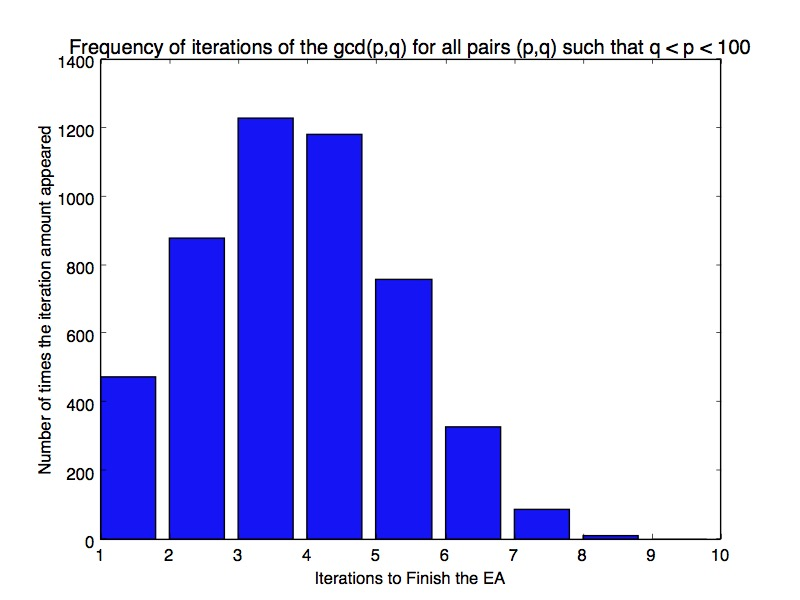
\includegraphics[scale=.45]{2digit_iterationfreq.jpg}
		\center \tiny(Figure 1)
		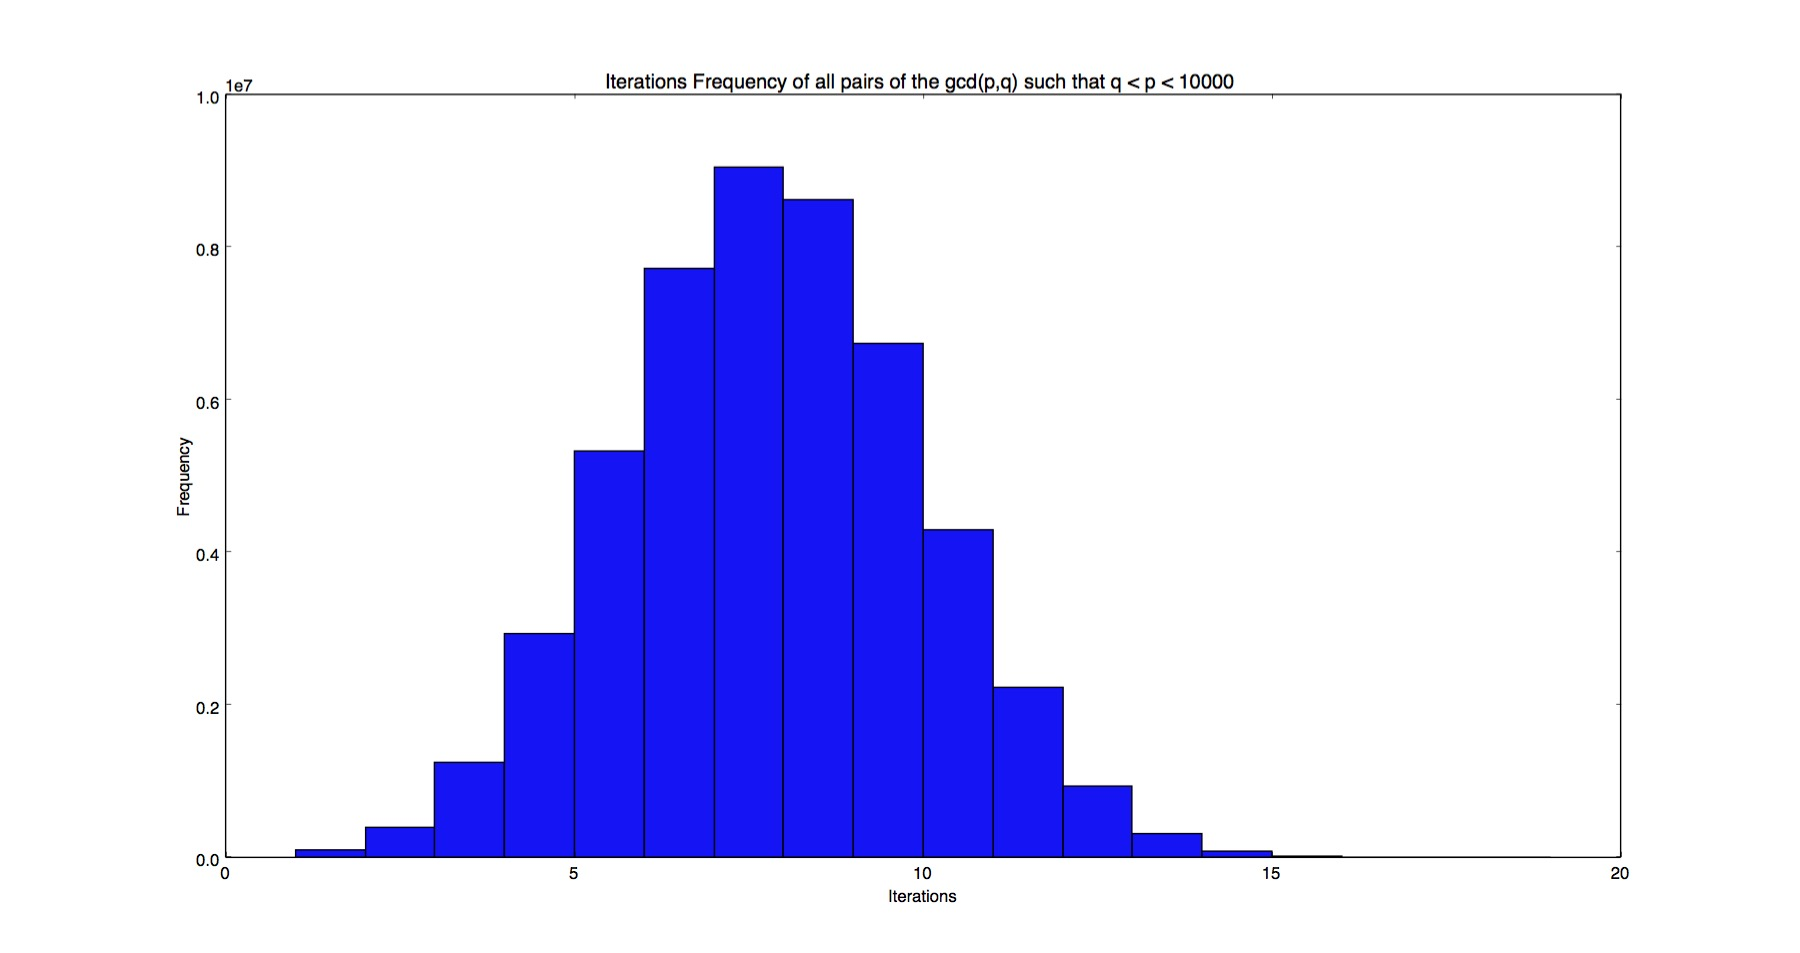
\includegraphics[scale=.45]{4digit_iteration_freq.jpg}
		\center \tiny(Figure 2)
	\end{figure}
	
	\begin{figure}
		\centering
		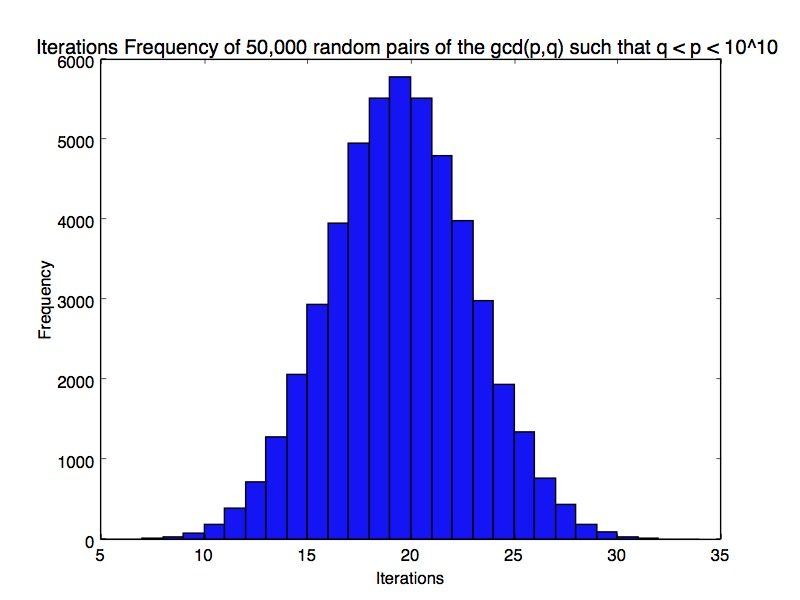
\includegraphics[scale=.45]{10_digit_numbers.jpg}
		\center \tiny(Figure 3)
			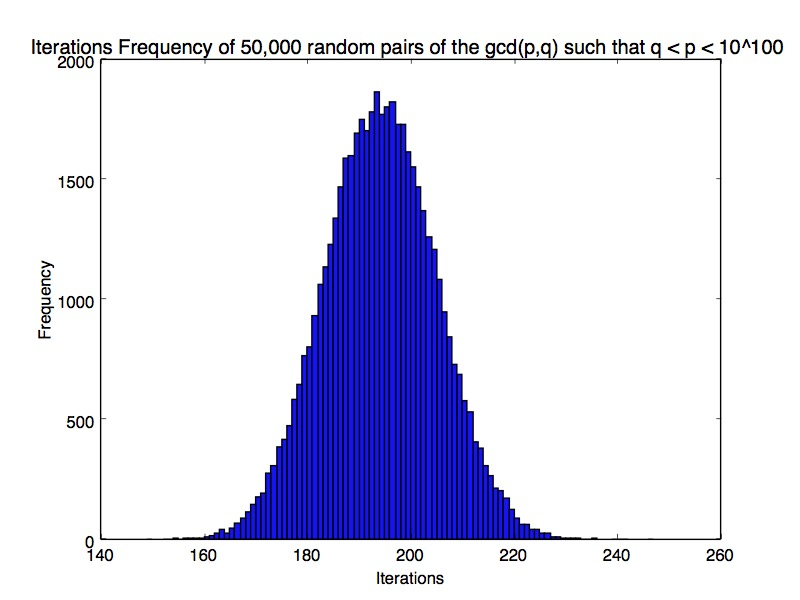
\includegraphics[scale=.45]{100_digit_numbers_freq.jpg}
		\center \tiny(Figure 4)
		
	\end{figure}
	
	
	
	\begin{figure}
		\centering

		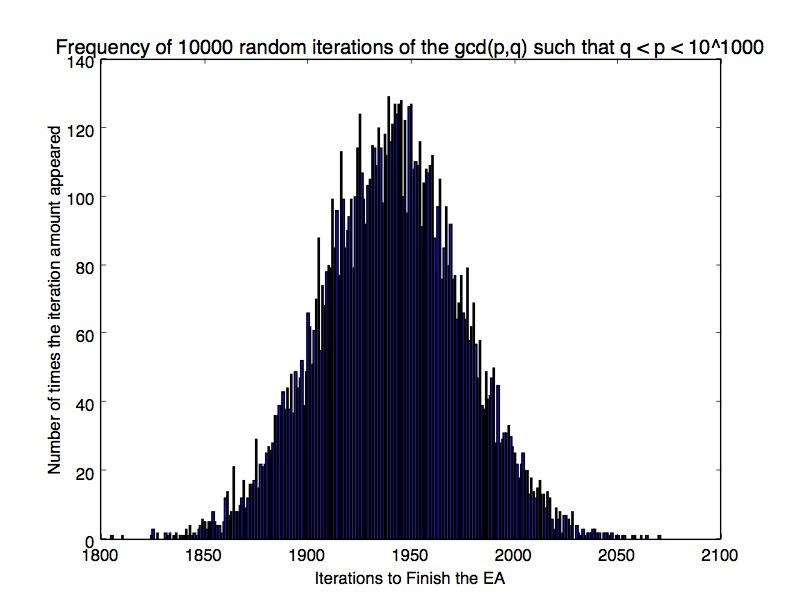
\includegraphics[scale=.45]{1000_digit_numbers.jpg}
		\center \tiny(Figure 5)
		
	\end{figure}
	\newpage
	As the number of digits we consider increases, the distribution	 becomes continuously more Gaussian. However, after a point our computational resources restrict us from checking all pairs p,q with some large upper bound. Thus, we restrict ourselves by picking a set amount of pairs and calculating their distribution. You can see this progression as the figures continue.\\
	
	There are a few minor observations to be made:\\
	
	 First, in (Figure $1$), it must be noted that the lack of normality here is due to the small sample size. The size of this data set was no more than $4950$, and spanned across $9$ bins. As the number of bins needed increases, the more normal the graph becomes. 
	
	 Second, in (Figure $5$), the inconsistencies in the normal distribution can be attributed to a too small a sample size. If given the computing power and time, one could compute all pairs less than $10^{1000}$. Note the increasing mean iterations as we climb the upper bound.
\section{Discussion}$ $
As it is obvious, the distribution of these gcd lengths is almost perfectly Gaussian. The approach we used seemed to work awfully well, as computers handle modular operations and subtraction very well. The main constraints we had were as we went past $5$ digit numbers. Calculating all pairs becomes exponentially difficult as the digits you allow increases. 



\section{Individual Contributions}$ $





\end{document}